\chapter{哺乳动物的有性生殖}\label{ch:b2:mammal-reproduction}

人类卵细胞直径约十分之一毫米，是人体中最大的细胞；
精子则是带有“螺旋桨”的细胞核，一次释放约三亿个，
其中仅几十个能到达卵细胞，
只有一个会进入其中。一周之内，受精卵
发育成中空的球体，钻入子宫壁，并
利用自身外层细胞构建器官——\omterm{def:b2:mammal-reproduction:placenta}{胎盘}——，
母体借此在九个月里为其提供营养。随后，它
出生，并以乳汁哺育。所有哺乳动物都如此，没有其他动物
能完成全部这些过程。本章依次讨论配子直至受精，
胚胎直至\omterm{def:b2:mammal-reproduction:implantation}{着床}，以及生物体经历妊娠、分娩
与哺乳的过程，最后讨论两性是如何形成的。

\section{性腺与配子}

\begin{definition}[睾丸与精子发生]\label{def:b2:mammal-reproduction:testis}
\index{精子发生}\index{生精小管}\index{支持细胞}\index{莱迪希细胞}
\emph{睾丸}由大量\emph{生精小管}组成，总长可达数百米，
其管壁产生精子；
小管之间分布着\emph{莱迪希细胞}，能合成睾酮。在生精小管壁中，
位于外缘的\emph{精原细胞}通过有丝分裂增殖，既维持干细胞群，
又将细胞向内输送；这些细胞逐渐长大，成为初级\emph{精母细胞}，
经减数第一次分裂形成两个次级精母细胞，
再经减数第二次分裂形成四个\omterm{def:b2:meiosis-heredity:meiosis}{单倍体}\emph{精细胞}；
精细胞舍弃大部分细胞质，使细胞核浓缩，长出鞭毛，
并在细胞核上覆盖由酶构成的小泡——\emph{顶体}，
最终成为释放到管腔中的\emph{精子}。
体积较大的\emph{支持细胞}贯穿管壁，为生殖细胞提供营养，
并通过相邻细胞之间的紧密连接形成\emph{血–睾屏障}，
使免疫系统无法接触青春期才出现的细胞。
整个过程在男性体内约需 \num{64} 天，
自青春期至老年，每天产生约 $10^{8}$ 个精子。
精子离开睾丸时尚不能运动，
之后在\emph{附睾}中成熟约两周。
\end{definition}

\begin{omfigure}
\begin{tikzpicture}[every node/.style={font=\scriptsize}]
  % tubule cross-section: concentric layers
  \draw[thick, fill=omExo!15] (0,0) circle (2.5);
  \draw[thick, fill=omExo!8] (0,0) circle (2.2);
  \draw[thick, fill=omDef!10] (0,0) circle (1.6);
  \draw[thick, fill=omProp!12] (0,0) circle (1.0);
  \draw[thick, fill=white] (0,0) circle (0.45);
  % cells
  \foreach \a in {0,30,...,330} \draw[thick, fill=omDef!40] (\a:2.0) circle (0.13);
  \foreach \a in {15,45,...,345} \draw[thick, fill=omDef!70] (\a:1.32) circle (0.16);
  \foreach \a in {0,20,...,340} \draw[thick, fill=omProp!60] (\a:0.75) circle (0.08);
  \foreach \a in {10,40,...,340} \draw[thick, omProp!80!black] (\a:0.45) -- (\a:0.15);
  % Sertoli cell: tall wedge
  \draw[thick, omExo!70!black, fill=omExo!40, opacity=0.6] (100:2.2) .. controls (90:1.6) and (95:0.9) .. (92:0.5) .. controls (80:0.9) and (75:1.6) .. (72:2.2) -- cycle;
  % Leydig cells outside
  \foreach \p in {(2.9,0.8),(3.1,0.3),(2.8,-0.3)} \draw[thick, fill=omThm!40] \p circle (0.14);
  % labels
  \draw (2.0,0) -- (3.6,-0.5) node[right, align=left] {精原细胞（$2n$）\\位于外缘};
  \draw (1.32,-0.7) -- (3.6,-1.5) node[right, align=left] {初级精母细胞 \\（减数第一次分裂）};
  \draw (0.75,-0.4) -- (3.6,-2.4) node[right, align=left] {精细胞（$n$）};
  \draw (0.3,-0.2) -- (3.6,-3.1) node[right, align=left] {管腔中的精子};
  \draw (2.95,0.55) -- (3.6,0.6) node[right, align=left] {莱迪希细胞：\\睾酮};
  \draw (88:1.4) -- (3.6,1.8) node[right, align=left] {贯穿管壁的支持细胞};
  \node[anchor=east, align=right] at (-2.7,0) {外侧 \\（基膜）};
\end{tikzpicture}

{\small \omterm{def:b2:mammal-reproduction:testis}{生精小管}的横切面。生殖细胞从外缘（精原细胞）向内逐步成熟
（精母细胞、精细胞、管腔中的精子），由\omterm{def:b2:mammal-reproduction:testis}{支持细胞}支撑；
位于小管之间的\omterm{def:b2:mammal-reproduction:testis}{莱迪希细胞}
合成睾酮。}
\end{omfigure}

\begin{omfigure}
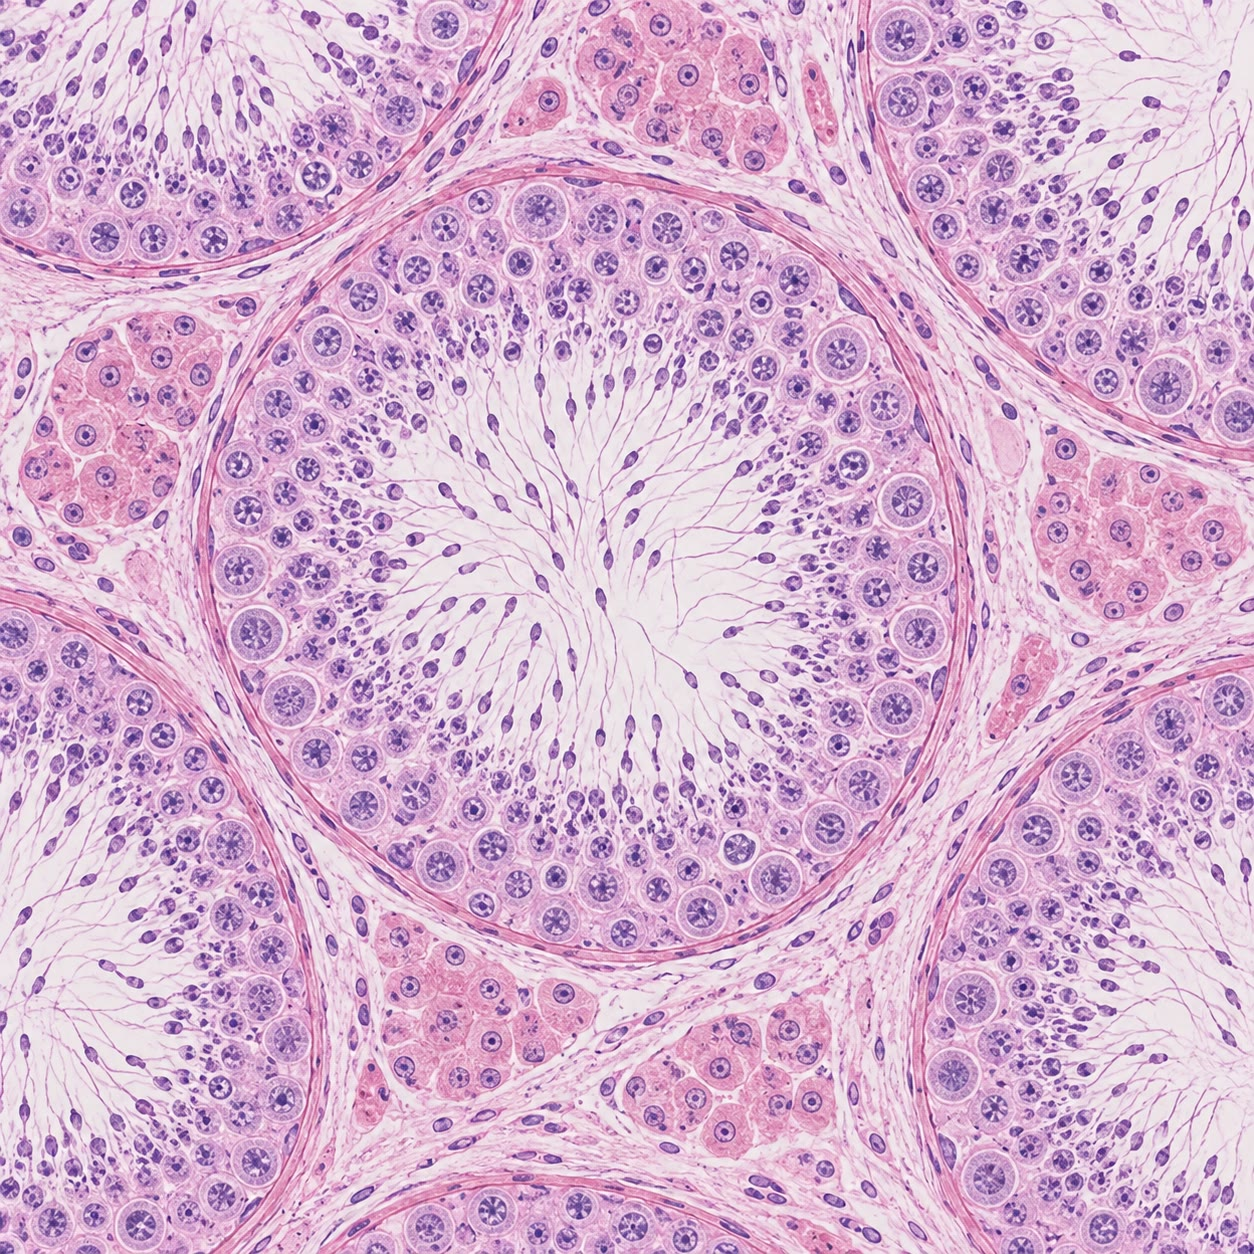
\includegraphics[width=0.42\linewidth]{images/book4/ai/b4-08-testis-histology.jpg}\hspace{0.04\linewidth}
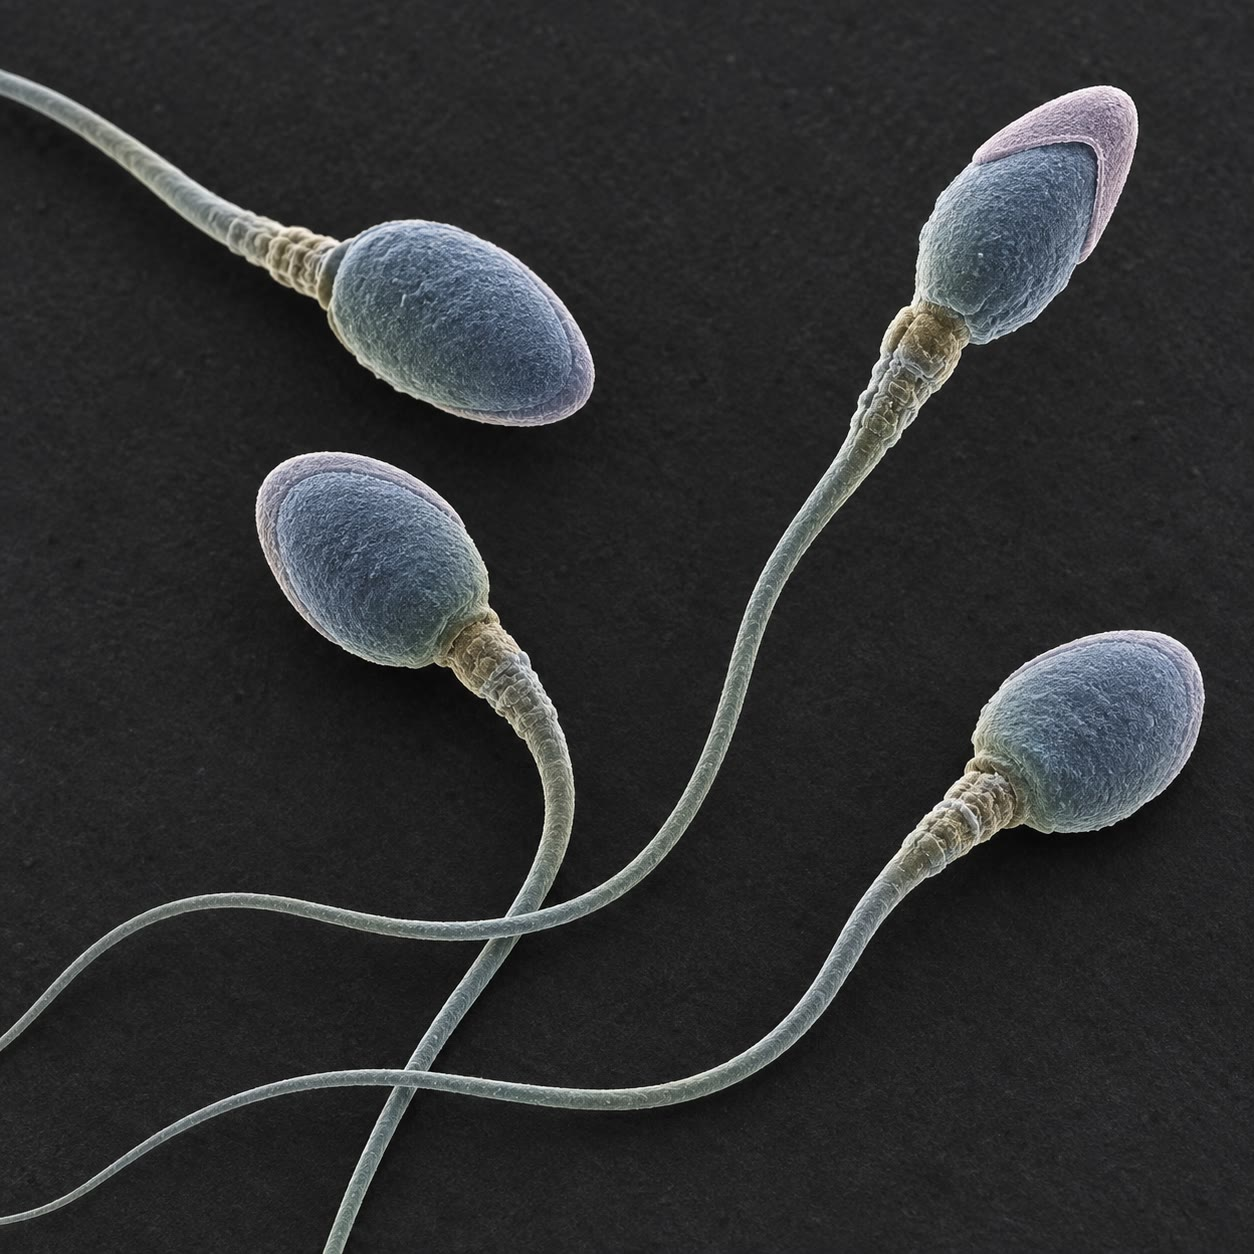
\includegraphics[width=0.42\linewidth]{images/book4/ai/b4-08-sperm-sem.jpg}

{\small 左：\omterm{def:b2:mammal-reproduction:testis}{生精小管}切片，
生殖细胞自管壁向管腔依次排列。
右：扫描电子显微镜下的精子，
可见头部的顶体帽。}
\end{omfigure}

\begin{definition}[卵巢与卵子发生]\label{def:b2:mammal-reproduction:ovary}
\index{卵子发生}\index{卵泡}\index{排卵}\index{黄体}
卵子发生与\omterm{def:b2:mammal-reproduction:testis}{精子发生}在几乎所有方面都如镜像般对应。
\emph{卵原细胞}只在胎儿期增殖；女孩出生时，
体内约有一百万个初级\emph{卵母细胞}，
每个都停滞于减数第一次分裂前期，
并被一层细胞包裹——即\emph{原始卵泡}——，此后再不产生新的卵母细胞。
自青春期起，每月都有一批卵泡开始发育：
卵母细胞增大，周围的\emph{颗粒层}细胞增殖形成多层，
外层形成\emph{卵泡膜}，
卵泡内出现充满液体的腔（即\emph{格拉夫卵泡}，直径可达两厘米），
通常只有一个卵泡发育至\emph{排卵}：此时卵母细胞才完成减数第一次分裂，
随后又停滞于减数第二次分裂中期，
连同周围的颗粒层细胞一起排入输卵管。
排空的卵泡转变为\emph{黄体}，这是一个暂时性的、分泌孕酮的腺体。
\omterm{def:b2:meiosis-heredity:meiosis}{减数分裂}产生一个卵细胞和三个极小的极体——
全部细胞质都进入一个细胞中——，减数第二次分裂
只有在精子进入后才会完成。在约一百万个卵母细胞中，
约 \num{400} 个会在一生中排出，其余则退化
（\emph{闭锁}）；卵母细胞储备耗尽时，约在五十岁左右，
月经周期停止，即绝经。
\end{definition}

\begin{omfigure}
\begin{tikzpicture}[every node/.style={font=\scriptsize}, >=stealth]
  % timeline of oogenesis vs spermatogenesis
  \draw[thick, ->] (0,3.0) -- (12.6,3.0); \node[anchor=west] at (12.6,3.0) {年龄};
  \foreach \x/\l in {0/{胎儿}, 2.2/{出生}, 4.6/{青春期}, 10.2/{约 50 岁}}
    \draw (\x,3.1) -- (\x,2.9) node[above=0.15cm] {\l};
  % oogenesis line
  \node[anchor=east, omThm] at (-0.2,1.5) {卵子发生};
  \draw[very thick, omThm] (0,1.5) -- (1.6,1.5); \node[above, omThm, align=center] at (0.8,1.55) {卵原细胞 \\增殖};
  \draw[very thick, omThm, dashed] (1.6,1.5) -- (4.6,1.5); \node[below, omThm] at (3.1,1.45) {停滞于减数第一次分裂前期};
  \draw[very thick, omThm] (4.6,1.5) -- (10.2,1.5); \node[above, omThm, align=center] at (7.4,1.55) {每月排卵一次；\\减数第一次分裂在排卵时完成，第二次在受精时完成};
  \fill[omThm] (10.2,1.5) circle (0.07); \node[below, omThm] at (10.2,1.45) {储备耗尽};
  % spermatogenesis line
  \node[anchor=east, omDef] at (-0.2,0.3) {精子发生};
  \draw[very thick, omDef, dashed] (0,0.3) -- (4.6,0.3); \node[above, omDef] at (2.3,0.35) {精原细胞静止};
  \draw[very thick, omDef, ->] (4.6,0.3) -- (12.6,0.3); \node[above, omDef] at (8.6,0.35) {持续进行：每天 $10^{8}$ 个精子，每个历时 64 天，来自干细胞};
\end{tikzpicture}

{\small 两种配子发生的时间进程。卵母细胞在出生前全部形成，
并从有限的储备中逐个释放；精子则在整个成年期
由干细胞持续产生。}
\end{omfigure}

\begin{omfigure}
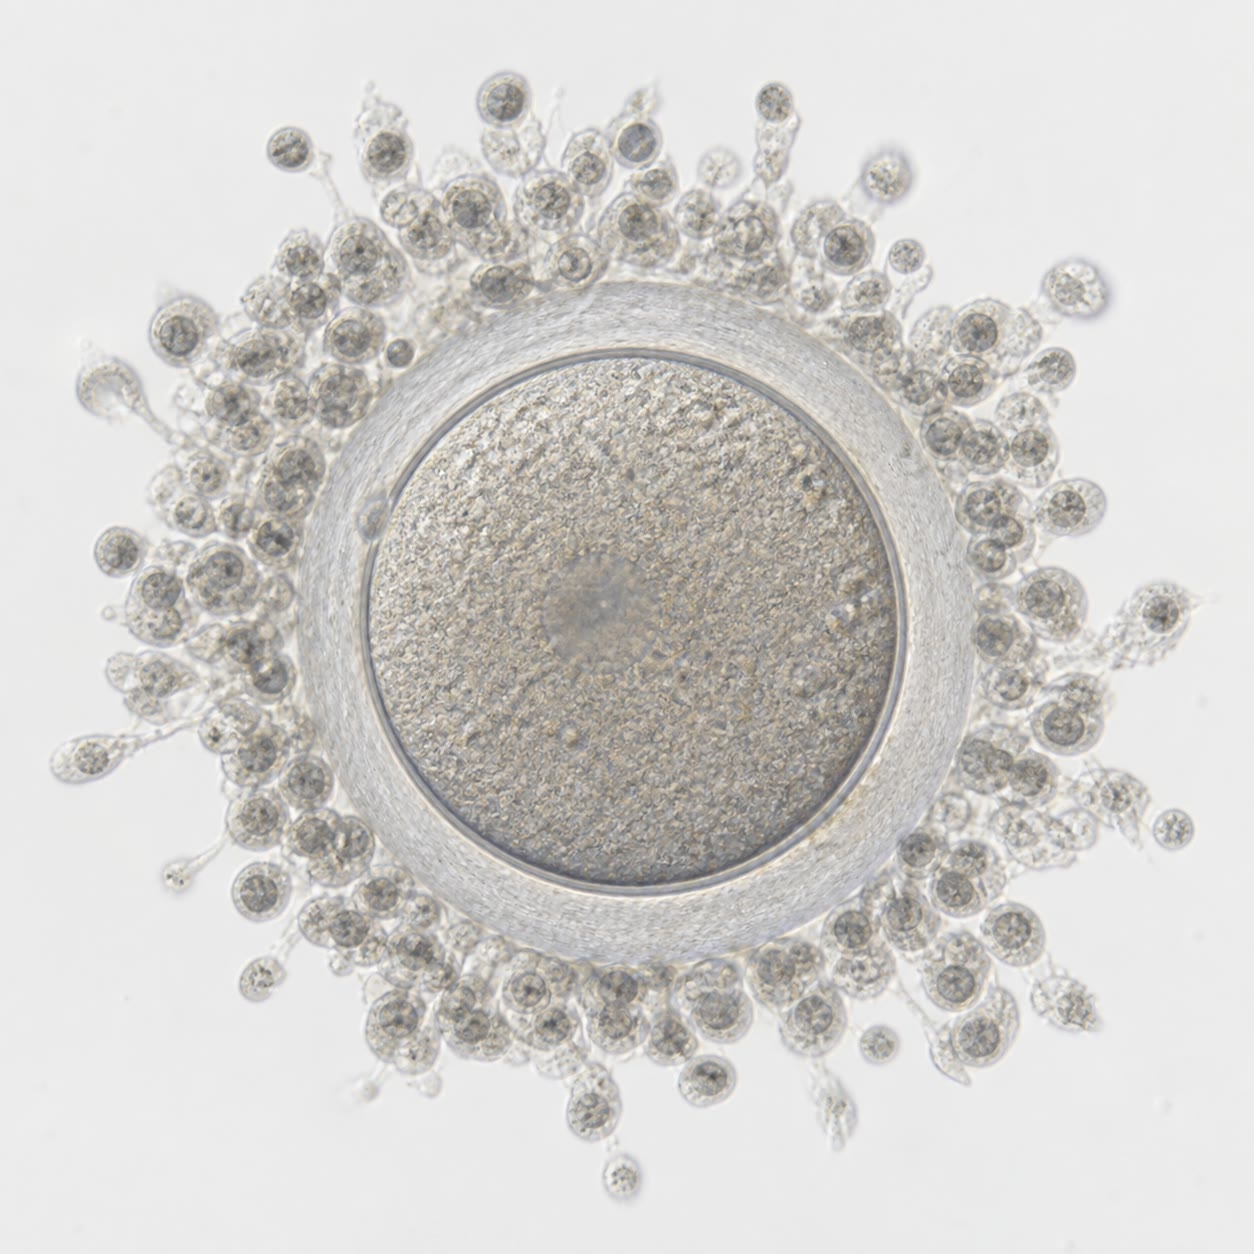
\includegraphics[width=0.46\linewidth]{images/book4/ai/b4-08-oocyte.jpg}

{\small \omterm{def:b2:mammal-reproduction:ovary}{排卵}后的卵母细胞：细胞本身、其透明的外被（
\omterm{prop:b2:mammal-reproduction:fertilisation}{透明带}），以及随之离开
\omterm{def:b2:mammal-reproduction:ovary}{卵泡}的颗粒层细胞群。}
\end{omfigure}

\section{受精}

\begin{proposition}[受精的各步骤]\label{prop:b2:mammal-reproduction:fertilisation}
\index{受精!哺乳动物}\index{顶体反应}\index{透明带}\index{皮质反应}
精子射入阴道——约 $3\times 10^{8}$ 个——穿过
宫颈黏液，借子宫收缩上行至子宫，
其中数百个在一小时内抵达输卵管壶腹部，
卵子在那里等待一天。精子在途中经历
\emph{获能}：雌性生殖道的分泌物使其膜上的
包被蛋白脱落，并使其活动增强。在卵子处，
一个精子穿过颗粒层细胞，与
\emph{\omterm{prop:b2:mammal-reproduction:fertilisation}{透明带}}的一种糖蛋白结合，并发生\emph{\omterm{prop:b2:mammal-reproduction:fertilisation}{顶体
反应}}，释放酶类，在\omterm{prop:b2:mammal-reproduction:fertilisation}{透明带}上消化出一条通道；
其膜与卵子膜融合，精子细胞核进入卵内。
卵子在数秒内作出反应：钙离子波扫过卵子，皮质
颗粒释放出酶，使\omterm{prop:b2:mammal-reproduction:fertilisation}{透明带}变硬，并去除其上的精子
受体——这便是\emph{\omterm{prop:b2:mammal-reproduction:fertilisation}{皮质反应}}，即阻止\omterm{thm:b2:mammal-reproduction:poisson}{多精受精}的机制。
卵子完成减数第二次分裂，排出第二极体，并
两个\omterm{def:b2:meiosis-heredity:meiosis}{单倍体}的\emph{原核}各自复制 DNA，相互靠拢并
进入第一次有丝分裂：受精卵已形成一天。物种
专一性取决于\omterm{prop:b2:mammal-reproduction:fertilisation}{透明带}蛋白，这就是为什么小鼠精子
不能进入人类卵子。
\end{proposition}
\begin{proof}[证据]
爱德华兹与斯特普托（1978）使一个人类卵母细胞受精，该卵母细胞
取自\omterm{def:b2:mammal-reproduction:ovary}{排卵}前不久的卵巢，在培养皿中与已获能的精子
共同培养，将胚胎培养至八细胞期后放回子宫，
胚胎在子宫内\omterm{def:b2:mammal-reproduction:implantation}{着床}并出生：即体外受精。
上述序列的每一步，最初都是在海胆和小鼠中
研究清楚的，其中融合、钙离子波和皮质颗粒释放
均可直接观察到；在小鼠中，通过\omterm{def:b2:genome-diversification:mutation}{突变}去除
一种\omterm{prop:b2:mammal-reproduction:fertilisation}{透明带}糖蛋白（ZP2 或 ZP3），得到的卵子
精子无法与之结合。
\end{proof}

\begin{theorem}[为什么一个卵子需要数百万个精子]\label{thm:b2:mammal-reproduction:poisson}
\index{多精受精}
若射入的 $N$ 个精子中，每个精子各自独立地
以较小的概率 $\pi$ 到达卵子表面，则到达的精子数
服从均值为 $m = N\pi$ 的泊松分布，且至少有一个
精子到达的概率为
\[
P = 1 - e^{-m}.
\]
当 $N = 3\times 10^{8}$ 且 $\pi \approx 10^{-8}$ 时，$m \approx 3$
$P \approx 0.95$；取 $N = 2\times 10^{7}$（临床
低精子数阈值）时，$m = 0.2$，$P = 0.18$。同样的
计算也说明了阻止\omterm{thm:b2:mammal-reproduction:poisson}{多精受精}的机制为何不可或缺：当
$P$ 较高时，数个精子会在数秒之内相继到达，
而一个被两个精子进入的卵子将成为三倍体并死亡。
\end{theorem}
\begin{proof}
每个精子是一次独立试验，成功概率为 $\pi$；
成功次数服从二项分布，当 $N$ 大、
$\pi$ 较小时，它近似为均值为 $N\pi$ 的泊松分布。零次
成功的概率为 $e^{-m}$，故至少一次成功的概率为 $1 - e^{-m}$；
两次或更多次成功的概率为 $1 - e^{-m}(1 + m)$，约
为 $0.8$（当 $m = 3$ 时）。
\end{proof}

\begin{omfigure}
\begin{tikzpicture}[every node/.style={font=\scriptsize}, >=stealth]
  \foreach \x/\lab in {0/{1. 精子结合 \\透明带}, 3.3/{2. 顶体反应：\\酶切开通路}, 6.6/{3. 质膜融合；\\钙波}, 9.9/{4. 皮质反应：\\透明带硬化，\\减数第二次分裂完成}} {
    \begin{scope}[xshift=\x cm]
      \draw[thick, fill=omThm!8] (0,0) circle (0.9);
      \draw[thick, omExo!70!black] (0,0) circle (1.15);
      \node[below, align=center] at (0,-1.3) {\lab};
    \end{scope}
  }
  % stage 1: sperm at zona
  \draw[thick, fill=omDef!50] (-1.45,0.1) ellipse (0.18 and 0.11); \draw[thick, omDef] (-1.63,0.1) .. controls (-2.0,0.4) and (-2.2,-0.2) .. (-2.5,0.1);
  % stage 2: sperm digging through zona
  \begin{scope}[xshift=3.3cm]
    \fill[white] (-1.2,0.0) circle (0.12);
    \draw[thick, fill=omDef!50] (-1.05,0.05) ellipse (0.18 and 0.11); \draw[thick, omDef] (-1.23,0.05) .. controls (-1.6,0.35) and (-1.8,-0.25) .. (-2.1,0.05);
    \foreach \a in {150,170,190,210} \draw[omProp, thick] (-1.2,0.0) -- ++(\a:0.25);
  \end{scope}
  % stage 3: fused, calcium wave
  \begin{scope}[xshift=6.6cm]
    \fill[white] (-1.15,0.0) circle (0.12);
    \draw[thick, fill=omDef!50] (-0.75,0.0) ellipse (0.18 and 0.11);
    \draw[thick, omDef] (-0.93,0.0) .. controls (-1.3,0.3) and (-1.5,-0.3) .. (-1.8,0.0);
    \foreach \r in {0.35,0.55,0.75} \draw[omProp, thick] (-0.75,0) ++(-60:\r) arc (-60:60:\r);
  \end{scope}
  % stage 4: hardened zona, polar body, pronuclei
  \begin{scope}[xshift=9.9cm]
    \draw[very thick, omExo!70!black] (0,0) circle (1.15);
    \draw[thick, fill=omDef!30] (-0.25,0.05) circle (0.2); \draw[thick, fill=omThm!30] (0.25,0.05) circle (0.2);
    \draw[thick, fill=omThm!20] (0.55,0.95) circle (0.12);
    \node[anchor=west] at (1.2,0.9) {极体};
    \draw (0.45,0.05) -- (1.2,-0.35); \node[anchor=west] at (1.2,-0.35) {两个原核};
  \end{scope}
\end{tikzpicture}

{\small 受精分为四步：与\omterm{prop:b2:mammal-reproduction:fertilisation}{透明带}结合、\omterm{prop:b2:mammal-reproduction:fertilisation}{顶体反应}、
融合与钙离子波，以及\omterm{prop:b2:mammal-reproduction:fertilisation}{皮质
反应}，它封闭卵子以阻止其他精子，同时卵子
完成\omterm{def:b2:meiosis-heredity:meiosis}{减数分裂}。}
\end{omfigure}

\section{着床与胎盘}

\begin{definition}[卵裂、囊胚与着床]\label{def:b2:mammal-reproduction:implantation}
\index{囊胚}\index{滋养层}\index{内细胞团}\index{着床}
受精卵每隔十二至二十小时分裂一次，
在沿输卵管下行的过程中并不生长（\emph{卵裂}）：
先为两个细胞，继而为四个、八个，
然后成为由十六个细胞组成的致密细胞球（\emph{桑葚胚}）。
到第五天时，形成约一百个细胞的\emph{囊胚}：外层为
\emph{滋养层}，环绕着一个囊腔，囊腔一侧有一团细胞，即
\emph{内细胞团}。滋养层将发育为\omterm{def:b2:mammal-reproduction:placenta}{胎盘}和胎膜，内细胞团
则将发育为胚胎——在这一阶段取出时，可获得胚胎干细胞。
第六天，囊胚从\omterm{prop:b2:mammal-reproduction:fertilisation}{透明带}中孵出，附着于子宫内膜，
滋养层随即侵入其中：细胞融合成一个多核的前沿结构，
分解母体组织并打开母体毛细血管，于是到第十二天，
胚胎已埋入子宫壁中，并浸浴在母体血液之中。这就是\emph{着床}。
着床只有在经孕酮准备好的子宫中才能成功，
且只发生在仅持续几天的窗口期内；
约有一半的人类受孕
会在此步骤之前或之时失败，通常由卵子的染色体错误所致。
\end{definition}

\begin{omfigure}
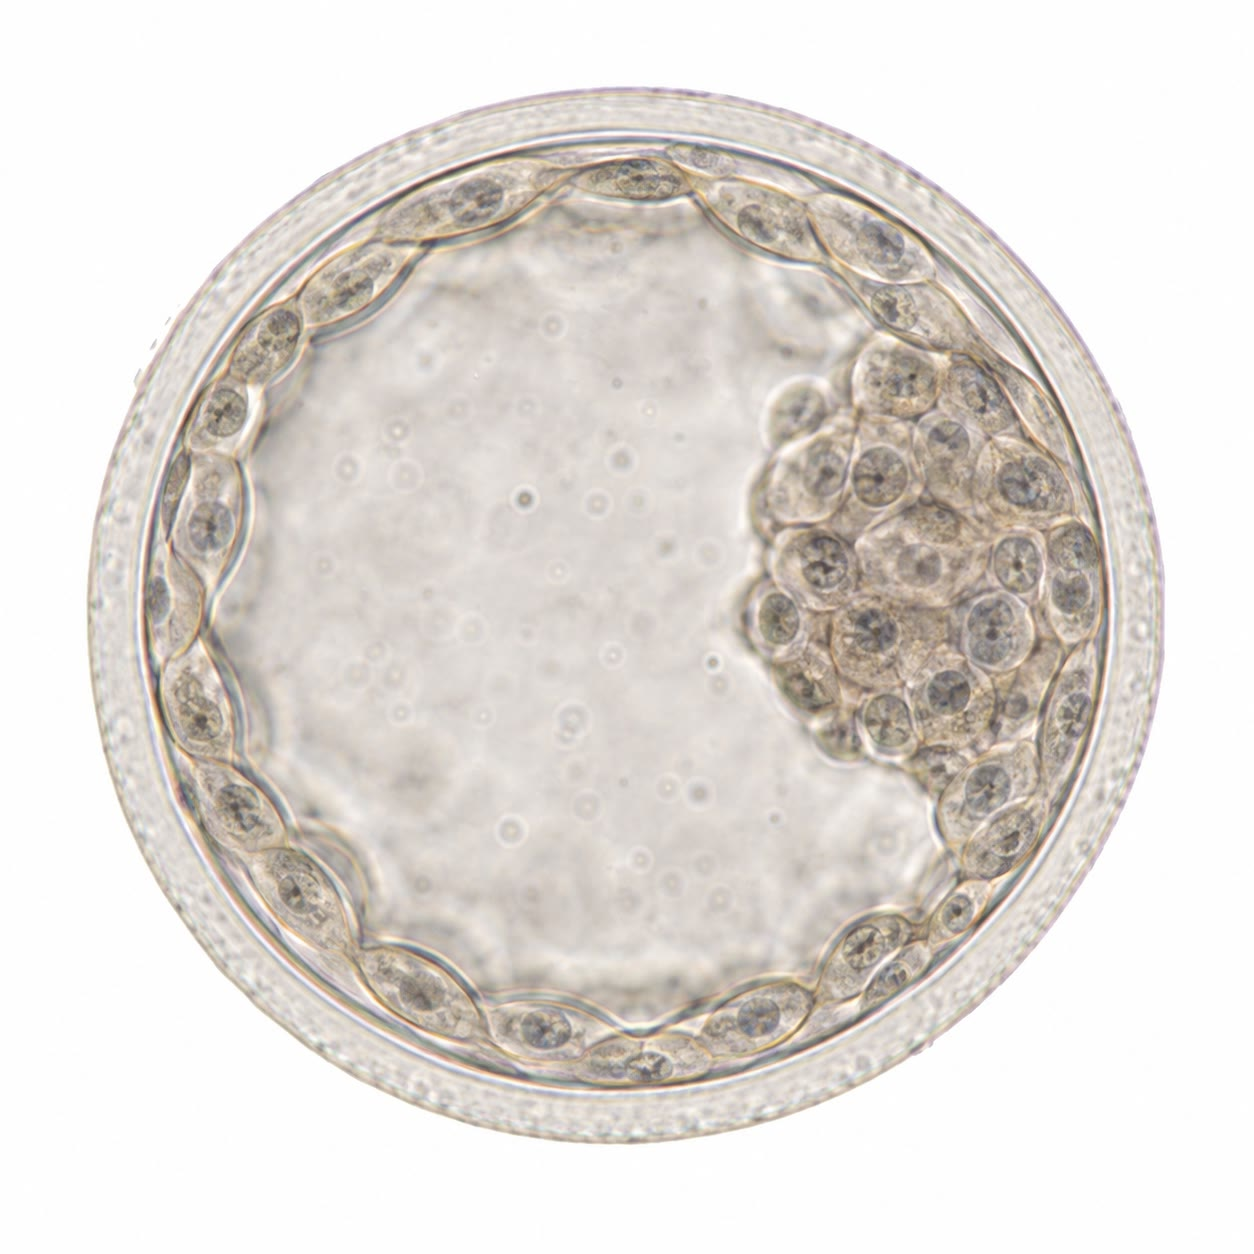
\includegraphics[width=0.42\linewidth]{images/book4/ai/b4-08-blastocyst.jpg}

{\small 第五天的\omterm{def:b2:mammal-reproduction:implantation}{囊胚}：外层的\omterm{def:b2:mammal-reproduction:implantation}{滋养层}环绕着
囊腔，\omterm{def:b2:mammal-reproduction:implantation}{内细胞团}——即未来的胚胎——位于
一侧。}
\end{omfigure}

\begin{definition}[胎盘]\label{def:b2:mammal-reproduction:placenta}
\index{胎盘}\index{绒毛膜绒毛}\index{脐带}
\emph{胎盘}是一个器官，
由胚胎（绒毛膜，来自\omterm{def:b2:mammal-reproduction:implantation}{滋养层}）与母体（子宫内膜）共同构成。
指状的\emph{绒毛膜绒毛}多级分支，足月时总表面积达
\qty{12}{m^2}，悬浮于由子宫动脉以每分钟半升输入的
母体血液湖中；每条绒毛内部有胎儿毛细血管，
经\emph{脐带}中的两条动脉和一条静脉与胎儿相连。
两种血液从不混合：它们之间隔着绒毛壁，
即几微米厚的\omterm{def:b2:mammal-reproduction:implantation}{滋养层}与毛细血管内皮，
氧气、$\mathrm{CO_2}$、水、尿素和脂溶性分子经此扩散，
葡萄糖与氨基酸
由转运蛋白运送，
母体抗体（IgG）则借助受体转运，
使新生儿在最初几个月获得免疫力。胎盘同时也是一个腺体：
从孕早期起，\omterm{def:b2:mammal-reproduction:implantation}{滋养层}即分泌\emph{人绒毛膜促性腺激素}
（hCG），维持\omterm{def:b2:mammal-reproduction:ovary}{黄体}继续分泌孕酮；
从第三个月起，胎盘自身分泌孕酮和雌激素，
以维持妊娠（见\cref{ch:b2:reproductive-hormones}）。
从效果上说，它是一个
为九个月而生长、出生时即被弃去的
肺、肠、肾和内分泌腺。
\end{definition}

\begin{omfigure}
\begin{tikzpicture}[every node/.style={font=\scriptsize}, >=stealth]
  % maternal blood space
  \fill[omThm!12] (0,0) rectangle (8,3.6);
  \node[omThm!80!black, align=center] at (1.1,2.6) {母体血液 \\（绒毛间隙）};
  % uterine wall at bottom
  \fill[omExo!30] (0,-0.6) rectangle (8,0); \node at (4,-0.3) {子宫壁（母体）};
  \draw[->, thick, omThm] (1.0,-0.6) -- (1.0,0.6); \node[omThm, anchor=west] at (1.05,0.3) {螺旋动脉};
  \draw[->, thick, omDef!60!black] (7.0,0.6) -- (7.0,-0.6); \node[omDef!60!black, anchor=east] at (6.95,0.3) {子宫静脉};
  % chorionic plate at top
  \fill[omDef!20] (0,3.6) rectangle (8,4.4); \node at (4,4.0) {绒毛膜板（胎儿）};
  % villi hanging down
  \foreach \x in {2.6,4.2,5.8} {
    \draw[thick, fill=omDef!8] (\x-0.35,3.6) -- (\x-0.4,1.4) .. controls (\x-0.4,0.9) and (\x+0.4,0.9) .. (\x+0.4,1.4) -- (\x+0.35,3.6);
    \draw[thick, omThm!70!black] (\x-0.15,3.6) -- (\x-0.15,1.5) .. controls (\x-0.15,1.25) and (\x+0.15,1.25) .. (\x+0.15,1.5) -- (\x+0.15,3.6);
    \foreach \y in {2.0,2.7} { \draw[thick, fill=omDef!8] (\x-0.4,\y) .. controls (\x-0.9,\y+0.1) and (\x-0.9,\y-0.4) .. (\x-0.4,\y-0.3); }
  }
  % umbilical vessels
  \draw[very thick, omThm!70!black] (4.2,4.4) -- (4.2,5.0) node[above, align=center] {脐静脉（通向胎儿）\\与脐动脉};
  \draw[very thick, omDef!60!black] (3.9,4.4) -- (3.9,5.0); \draw[very thick, omDef!60!black] (4.5,4.4) -- (4.5,5.0);
  % exchange arrows
  \draw[<->, thick] (3.0,2.2) -- (3.75,2.2); \node[anchor=west, align=left] at (8.3,1.5) {穿过绒毛壁：\textcolor{omThm}{O$_2$、葡萄糖、}\\\textcolor{omThm}{氨基酸、IgG}流向胎儿；\\\textcolor{omDef!60!black}{CO$_2$、尿素}流向母体};
  \node[anchor=west, align=left] at (8.3,3.0) {绒毛壁：滋养层 \\+胎儿毛细血管内皮，\\厚几微米};
  \draw (6.2,2.5) -- (8.3,3.0);
\end{tikzpicture}

{\small \omterm{def:b2:mammal-reproduction:placenta}{胎盘}：胎儿绒毛内含胎儿毛细血管，悬浮于
充满来自螺旋动脉的母体血液的空间中。两种血液在
绒毛壁处进行交换，但从不混合。}
\end{omfigure}

\begin{theorem}[胎盘的交换]\label{thm:b2:mammal-reproduction:fick}
\index{菲克定律!胎盘}
气体穿过面积为 $A$、厚度为 $d$ 的膜时，速率为
$J = K\,A\,\Delta P/d$，其中 $\Delta P$ 为其分压之差，$K$ 为组织的
通透性。对于组织中的氧气，
$K \approx \qty{3e-8}{mL/(cm.min.mmHg)}$；取 $A =
\qty{12}{m^2}$、$d = \qty{3.5}{\micro m}$、$\Delta P =
\qty{20}{mmHg}$（绒毛间隙中母体为 \qty{40}{mmHg}，
脐动脉中为 \qty{20}{mmHg}），\omterm{def:b2:mammal-reproduction:placenta}{胎盘}每分钟可转运约
\qty{200}{mL} 氧气，约为足月胎儿
每分钟耗氧量 \qty{25}{mL/min} 的八倍。因此，氧气的转运并非受扩散限制，
而是受血流限制。胎儿在较低的氧分压下工作，
并以亲和力更高的血红蛋白
和更高的红细胞数加以补偿。
\end{theorem}
\begin{proof}
菲克定律指出，通量与梯度
$\Delta P/d$ 及面积成正比；常数 $K$ 吸收了该气体在组织中的溶解度
与扩散系数。数值计算如下：
$3\times 10^{-8}\times 1.2\times 10^{5}\times 20/(3.5\times 10^{-4})
= \qty{206}{mL/min}$，其中 $A$ 以 \unit{cm^2} 计，$d$ 以 \unit{cm} 计。
胎儿的需求量约为每千克每分钟 \qty{7}{mL}，
以体重 \qty{3.5}{kg} 计。
\end{proof}

\section{妊娠、分娩与泌乳}

\begin{proposition}[妊娠与分娩]\label{prop:b2:mammal-reproduction:birth}
\index{妊娠}\index{分娩}\index{催产素}
妊娠期在小鼠中持续 \num{20} 天，在人类中持续 \num{280} 天，在大象中持续 \num{660}
天——大致与体重的四分之一次方相当，
灵长类相对其体型而言偏慢。妊娠由孕酮维持，
孕酮使子宫肌保持安静，并使子宫颈保持闭合。\emph{分娩}
由胎儿自身启动：其肾上腺
皮质醇于足月时升高，使\omterm{def:b2:mammal-reproduction:placenta}{胎盘}由孕酮转为分泌雌激素，
雌激素使子宫获得\omterm{prop:b2:mammal-reproduction:birth}{催产素}受体，并
形成缝隙连接，启动前列腺素的释放。随后，
\emph{正反馈}接管：胎头压迫子宫颈，感觉神经
向下丘脑发出信号，\emph{\omterm{prop:b2:mammal-reproduction:birth}{催产素}}由
垂体后叶释放，子宫收缩，胎头压迫加剧；
循环不断增强，直至分娩，分娩后刺激消失，
循环随之停止——生理学中为数不多的正反馈之一，
而且它必须以一个事件告终。\omterm{def:b2:mammal-reproduction:placenta}{胎盘}
在数分钟后娩出。
\end{proposition}
\begin{proof}[证据]
弗格森（1941 年）在兔子身上证明，扩张子宫颈
会引起子宫收缩，而切断脊髓或
摘除垂体后叶均会消除该反应：这是一条
神经内分泌反射，由子宫颈经垂体至子宫。\omterm{prop:b2:mammal-reproduction:birth}{催产素}，
由杜维尼奥于 1953 年分离并人工合成，现已成为
引产的标准药物。
\end{proof}

\begin{proposition}[泌乳]\label{prop:b2:mammal-reproduction:lactation}
\index{泌乳}\index{催乳素}\index{乳汁}
乳腺是一种经过改造的汗腺，妊娠期间由
雌激素、孕酮和\omterm{prop:b2:mammal-reproduction:lactation}{催乳素}促其发育，但受孕酮抑制而
不分泌；\omterm{def:b2:mammal-reproduction:placenta}{胎盘}娩出后，孕酮水平下降，
在垂体前叶分泌的\emph{\omterm{prop:b2:mammal-reproduction:lactation}{催乳素}}作用下，
腺泡开始产生乳汁。该过程由两种反射推动：吮吸
刺激\omterm{prop:b2:mammal-reproduction:lactation}{催乳素}释放（维持乳汁合成并抑制\omterm{def:b2:mammal-reproduction:ovary}{排卵}），
以及\omterm{prop:b2:mammal-reproduction:birth}{催产素}释放（使腺泡周围的细胞收缩，
将乳汁挤出）。人乳约含
\qty{7}{\%} 乳糖、\qty{4}{\%} 脂肪、\qty{1}{\%} 蛋白质，
能量为 \qty{2.9}{kJ/mL}；产后最初几天的\emph{初乳}富含
抗体（IgA），可包裹婴儿的肠道。母亲每天约分泌
\qty{750}{mL} 乳汁，耗能约 \qty{2.5}{MJ}，约占其食物的四分之一，
且需持续数月；\omterm{prop:b2:mammal-reproduction:lactation}{泌乳}是哺乳动物生殖中最耗能的
环节，也是哺乳动物纲得名之处。
\end{proposition}

\section{两性的形成}

\begin{proposition}[性别决定与分化]\label{prop:b2:mammal-reproduction:sex}
\index{SRY}\index{抗缪勒管激素}\index{性别分化}
直到第六周，无论性别，人类胚胎都具有相同的
结构：未分化的性腺、两对导管（\emph{沃尔夫管}
和\emph{缪勒管}）以及中性的外生殖器。Y 染色体上的基因
\emph{\omterm{prop:b2:mammal-reproduction:sex}{SRY}}在性腺中开启，
使其发育为\omterm{def:b2:mammal-reproduction:testis}{睾丸}；若无此基因，性腺则发育为卵巢。胎儿
\omterm{def:b2:mammal-reproduction:testis}{睾丸}随后做两件事：其\omterm{def:b2:mammal-reproduction:testis}{支持细胞}分泌
\emph{\omterm{prop:b2:mammal-reproduction:sex}{抗缪勒管激素}}，使缪勒管
退化；其\omterm{def:b2:mammal-reproduction:testis}{莱迪希细胞}分泌\emph{睾酮}，
使沃尔夫管得以保留（将发育为附睾、输精管，
精囊），睾酮在转化为二氢睾酮后，塑造
外生殖器，形成阴茎与阴囊。若两种信号
皆缺失，沃尔夫管退化，缪勒管发育为
输卵管、子宫和阴道上段，外生殖器发育为
女性形态。女性途径是在无任何信号时所走的路径：
男性途径则须由\omterm{def:b2:mammal-reproduction:testis}{睾丸}主动施加，每一个
施加失败的环节——例如 \omterm{prop:b2:mammal-reproduction:sex}{SRY} \omterm{def:b2:genome-diversification:mutation}{突变}、缺乏激素
受体——都会产生染色体为 XY、\omterm{def:b2:meiosis-heredity:vocabulary}{表型}为女性或中间型
的个体。
\end{proposition}
\begin{proof}[证据]
乔斯特（1947 年）在兔胎儿的子宫内摘除其性腺，
此时导管尚未分化：无论染色体性别如何，
被去势的胎儿均发育出子宫、输卵管和女性生殖器。
将睾酮结晶植入被去势的胎儿，
可使该侧的沃尔夫管得以保留，但未能消除
缪勒管；移植的胎儿\omterm{def:b2:mammal-reproduction:testis}{睾丸}则两者兼顾，且作用限于同侧：
\omterm{def:b2:mammal-reproduction:testis}{睾丸}必须分泌第二种因子以抑制雌性导管，
该因子在三十年后被鉴定为\omterm{prop:b2:mammal-reproduction:sex}{抗缪勒管
激素}。此后，Y 染色体上一小段的性别逆转效应
将开关定位于\emph{\omterm{prop:b2:mammal-reproduction:sex}{SRY}}（1990 年）；一只 XX 小鼠
仅凭\emph{Sry}基因便发育为雄性。
\end{proof}

\begin{omfigure}
\begin{tikzpicture}[every node/.style={font=\scriptsize}, >=stealth]
  \node[draw, rounded corners, fill=omExo!25, align=center] (g) at (0,0) {未分化性腺 \\两套导管系统};
  \node[draw, rounded corners, fill=omDef!15, align=center] (t) at (4.2,1.4) {睾丸 \\（有 \emph{SRY}）};
  \node[draw, rounded corners, fill=omThm!15, align=center] (o) at (4.2,-1.4) {卵巢 \\（无 \emph{SRY}）};
  \node[draw, rounded corners, fill=omDef!15, align=center] (amh) at (8.6,2.3) {AMH：缪勒管退化};
  \node[draw, rounded corners, fill=omDef!15, align=center] (tst) at (8.6,0.6) {睾酮：保留沃尔夫管；\\DHT：男性外生殖器};
  \node[draw, rounded corners, fill=omThm!15, align=center] (f) at (8.6,-1.4) {无信号：沃尔夫管退化，\\缪勒管$\to$输卵管、子宫；\\女性外生殖器};
  \draw[->, thick] (g) -- (t); \draw[->, thick] (g) -- (o);
  \draw[->, thick] (t) -- (amh); \draw[->, thick] (t) -- (tst); \draw[->, thick] (o) -- (f);
\end{tikzpicture}

{\small \omterm{prop:b2:mammal-reproduction:sex}{性别分化}：由\emph{\omterm{prop:b2:mammal-reproduction:sex}{SRY}}形成的\omterm{def:b2:mammal-reproduction:testis}{睾丸}，
以两种激素施加男性途径；缺少两者时机体
发育为女性。}
\end{omfigure}

\section{练习}

\begin{exercise}[$\star$]\label{exo:b2:mammal-reproduction:1}
比较\omterm{def:b2:mammal-reproduction:testis}{精子发生}与\omterm{def:b2:mammal-reproduction:ovary}{卵子发生}：干细胞分裂时，
一次\omterm{def:b2:meiosis-heredity:meiosis}{减数分裂}产生多少个配子，一个配子需要多长时间形成，
两者的停滞发生在何处，以及一生中各能产生多少个
配子。
\end{exercise}

\begin{exercise}[$\star$]\label{exo:b2:mammal-reproduction:2}
列出从精子到达\omterm{prop:b2:mammal-reproduction:fertilisation}{透明带}至第一次有丝分裂之间的受精各步骤，
并说明哪一步阻止\omterm{thm:b2:mammal-reproduction:poisson}{多精受精}。
\end{exercise}

\begin{exercise}[$\star$]\label{exo:b2:mammal-reproduction:3}
写出\omterm{def:b2:mammal-reproduction:implantation}{囊胚}中的两类细胞群，以及各自的
去向。\omterm{def:b2:mammal-reproduction:implantation}{着床}从哪一天开始？为子宫做好准备的
必定是哪种激素？
\end{exercise}

\begin{exercise}[$\star$]\label{exo:b2:mammal-reproduction:4}
对下列各物质，说明其是否穿过\omterm{def:b2:mammal-reproduction:placenta}{胎盘}，以及
穿过的方式：氧气、葡萄糖、母体红细胞、IgG 抗体、尿素、
酒精、大多数细菌。
\end{exercise}

\begin{exercise}[$\star\star$]\label{exo:b2:mammal-reproduction:5}
已知每个精子的受精概率为 $\pi = 10^{-8}$，计算精子数为
$3\times 10^{8}$、$10^{8}$、
$4\times 10^{7}$ 和 $10^{7}$ 时的受精概率。精子数为何值时
受精概率降至一半以下？这说明生育力随精子数变化的剂量–反应关系
呈何种形状？
\end{exercise}

\begin{exercise}[$\star\star$]\label{exo:b2:mammal-reproduction:6}
一名女孩出生时有 $10^{6}$ 个卵母细胞，青春期（13 岁）时有 \num{300000} 个，
50 岁时约剩 \num{1000} 个，其间已\omterm{def:b2:mammal-reproduction:ovary}{排卵} \num{400} 个。
计算青春期前后卵母细胞闭锁的平均速率（每天损失的卵
母细胞数），并与\omterm{def:b2:mammal-reproduction:ovary}{排卵}速率相比较。
\end{exercise}

\begin{exercise}[$\star\star$]\label{exo:b2:mammal-reproduction:7}
胎儿血红蛋白的半饱和压 $P_{50} =
\qty{19}{mmHg}$，成人血红蛋白为 \qty{27}{mmHg}；取
饱和度 $S = P^{n}/(P_{50}^{n} + P^{n})$，其中 $n = 2.7$。
计算两者在 \qty{30}{mmHg}（脐静脉中的压强）下的饱和度，
并解释其优势。
\end{exercise}

\begin{exercise}[$\star\star$]\label{exo:b2:mammal-reproduction:8}
hCG 于\omterm{def:b2:mammal-reproduction:implantation}{着床}时（受精后第 7 天）出现在母体血液中，
浓度约为 \qty{1}{IU/L}，每两天翻一番；妊娠试验
可检出 \qty{25}{IU/L}。试验在受精后第几天
转为阳性？自末次月经起算，
第几天转为阳性（\omterm{def:b2:mammal-reproduction:ovary}{排卵}于第 14 天）？
\end{exercise}

\begin{exercise}[$\star\star$]\label{exo:b2:mammal-reproduction:9}
重新计算定理中的\omterm{def:b2:mammal-reproduction:placenta}{胎盘}氧转运量，设\omterm{def:b2:mammal-reproduction:placenta}{胎盘}面积为
\qty{6}{m^2}、绒毛壁厚为 \qty{10}{\micro m}，如某些病理情形，
并与胎儿需求比较，胎儿会
发生什么？
\end{exercise}

\begin{exercise}[$\star\star\star$]\label{exo:b2:mammal-reproduction:10}
预测下列胎儿的生殖管道系统与外生殖器：（a）XY 胎儿，
其细胞缺乏睾酮受体；（b）XY 胎儿缺乏
抗苗勒管激素；（c）XX 胎儿受到来自肾上腺的高浓度睾酮
作用；（d）XX 胎儿的一条 X 染色体上携带
\emph{\omterm{prop:b2:mammal-reproduction:sex}{SRY}}。请依据约斯特的结果逐一解释。
\end{exercise}

\begin{exercise}[$\star\star\star$]\label{exo:b2:mammal-reproduction:11}
同卵双胞胎产生于胚胎的分裂。若分裂发生在
第 3 天之前，双胞胎各有独立的\omterm{def:b2:mammal-reproduction:placenta}{胎盘}和羊膜囊；第 4 至 8 天之间，
则为一个\omterm{def:b2:mammal-reproduction:placenta}{胎盘}和两个羊膜囊；第 8 至 13 天之间，则为一个\omterm{def:b2:mammal-reproduction:placenta}{胎盘}和
一个羊膜囊；较晚分裂则为联体。在一组同卵双胞胎中，
\qty{30}{\%} 有独立\omterm{def:b2:mammal-reproduction:placenta}{胎盘}，\qty{68}{\%} 为一个\omterm{def:b2:mammal-reproduction:placenta}{胎盘}和
两个羊膜囊，\qty{2}{\%} 为一个羊膜囊。试推断最常发生分裂的
发育阶段，并结合\omterm{def:b2:mammal-reproduction:implantation}{囊胚}解释每种情形下哪些
结构是共用的。
\end{exercise}

\begin{exercise}[$\star\star\star$]\label{exo:b2:mammal-reproduction:12}
有袋类经过数周即产下豆粒大小的幼体，
幼体在育儿袋内的乳头上完成生长；有\omterm{def:b2:mammal-reproduction:placenta}{胎盘}哺乳动物
妊娠期长，产下体型较大的幼体。比较这两种策略的
母体代价、风险，以及母体在不良季节放弃一窝幼崽的
能力方面有何差异，并推测为何有\omterm{def:b2:mammal-reproduction:placenta}{胎盘}哺乳动物
已在除澳大利亚外的各大洲取代了有袋类。
\end{exercise}

\section{问题：以数字看一次妊娠}

\begin{problem}[{周末问题——追踪一次人类妊娠，从精子
到乳汁，依次涉及受精概率、着床时间及其激素、
胎盘的交换能力、妊娠与泌乳的能量代价，
最终求出受精概率、试验转阳的日期、
胎盘的氧气余量，
以及一天乳汁的能量代价}]
\label{pb:b2:mammal-reproduction:1}
数据：每次射精含 $3\times 10^{8}$ 个精子，每个精子到达卵子
的概率为 $10^{-8}$；精子游动速度为 \qty{50}{\micro m/s}；
输卵管壶腹距宫颈 \qty{15}{cm}。\omterm{def:b2:mammal-reproduction:implantation}{着床}时（第 7 天）hCG 为
\qty{1}{IU/L}，每 \qty{2}{d} 翻一番；试验阈值为
\qty{25}{IU/L}。足月\omterm{def:b2:mammal-reproduction:placenta}{胎盘}：面积 \qty{12}{m^2}，绒毛壁
厚 \qty{3.5}{\micro m}，$K_{\mathrm{O_2}} = \qty{3e-8}{mL/(cm.min.mmHg)}$，
$\Delta P = \qty{20}{mmHg}$；胎儿体重 \qty{3.5}{kg}，每分钟每千克消耗
\qty{7}{mL} 氧气；母体\omterm{def:b2:mammal-reproduction:placenta}{胎盘}
血流量为 \qty{500}{mL/min}，每
毫升血液携带 \qty{0.16}{mL} 氧气。葡萄糖：胎儿每千克
每分钟消耗 \qty{5}{mg}；母体血液中为 \qty{0.9}{g/L}。乳汁：\qty{750}{mL/d}，
能量为 \qty{2.9}{kJ/mL}，制备效率为 \qty{80}{\%}；婴儿
每天增加 \qty{30}{g/d} 组织（沉积时每克 \qty{6}{kJ/g}），
维持能耗为 \qty{300}{kJ/kg/d}，体重为 \qty{4}{kg}。

\medskip
\noindent\textbf{第一部分——受精。}
\begin{enumerate}
  \item 计算到达卵子的精子平均数，以及
        受精概率。
  \item 计算两个或更多精子到达卵子的概率，并说明
        若无\omterm{prop:b2:mammal-reproduction:fertilisation}{皮质反应}，将会发生什么。
  \item 一个精子游到输卵管壶腹需要多长时间？精子
        在 \qty{30}{min} 内即可在该处发现：是什么将它们带到那里？
  \item 只有几百个精子到达输卵管壶腹。这占整次射精精子数的
        多大比例？其余精子在何处丢失？
  \item 卵子可受精的时间约为一天，精子在生殖道内
        可存活约三天。在一个周期中，有多少天的性交
        可能导致受孕？
  \item 某男子的精子数降至 $5\times 10^{7}$，重新计算
        每周期的受精概率，以及
        受孕所需周期数的期望值（几何分布）。
  \item 解释为何是卵子而非精子向胚胎提供
        胚胎的线粒体。
\end{enumerate}

\medskip
\noindent\textbf{第二部分——\omterm{def:b2:mammal-reproduction:implantation}{着床}及其激素。}
\begin{enumerate}[resume]
  \item 若每次卵裂各需
        \qty{16}{h}，到第 5 天时已经历多少次卵裂？共有多少个细胞？
  \item hCG 在受精后第几天
        达到检测阈值？从末次月经算起又是第几天（\omterm{def:b2:mammal-reproduction:ovary}{排卵}在第 14 天）？
  \item 为何 hCG 必须在\omterm{def:b2:mammal-reproduction:implantation}{着床}后数日内出现？
        若不出现，\omterm{def:b2:mammal-reproduction:ovary}{黄体}将发生何种变化，
        妊娠又会怎样？
  \item hCG 在约第 10 周时在 \qty{1e5}{IU/L} 附近达到峰值，随后下降。
        从\omterm{def:b2:mammal-reproduction:implantation}{着床}起，这相当于经历了多少次倍增，
        为何此后可以下降而妊娠不受影响？
  \item 半数受孕在\omterm{def:b2:mammal-reproduction:implantation}{着床}前或\omterm{def:b2:mammal-reproduction:implantation}{着床}时丢失，
        大多源于非整倍性的卵子。
        试利用\omterm{def:b2:mammal-reproduction:ovary}{卵子发生}的时间线，解释为何
        非整倍性在卵子中比在精子中更常见。
  \item 双胞胎：胚胎在第 6 天分裂。试说明两者
        是否共用\omterm{def:b2:mammal-reproduction:placenta}{胎盘}和羊膜囊。
\end{enumerate}

\medskip
\noindent\textbf{第三部分——\omterm{def:b2:mammal-reproduction:placenta}{胎盘}。}
\begin{enumerate}[resume]
  \item 计算最大扩散氧转运量。
  \item 计算胎儿的需氧量及扩散余量。
  \item 计算母体血流每分钟输送到\omterm{def:b2:mammal-reproduction:placenta}{胎盘}的氧量，
        为满足胎儿的需求，须提取其中的
        多大比例？
  \item 计算胎儿每日的葡萄糖需求量（以克计），以及
        含有这些葡萄糖的母体血液体积，并与
        母体每日流经\omterm{def:b2:mammal-reproduction:placenta}{胎盘}的血流量作比较。
  \item 胎儿血液离开\omterm{def:b2:mammal-reproduction:placenta}{胎盘}时的氧分压为
        \qty{30}{mmHg}。为何胎儿在这样的压强下不会窒息，而
        成人在此压强下会失去意识？
  \item 举出\omterm{def:b2:mammal-reproduction:placenta}{胎盘}在当时能完成、而胚胎的其他器官
        均无法完成的两项功能，以及\omterm{def:b2:mammal-reproduction:placenta}{胎盘}无法完成的一项功能。
\end{enumerate}

\medskip
\noindent\textbf{第四部分——分娩与乳汁。}
\begin{enumerate}[resume]
  \item 描述分娩过程中的正反馈，并解释它为何
        不会在足月前失控。
  \item 计算一日乳汁所含的能量，以及
        母体为产生乳汁所消耗的能量。
  \item 计算婴儿每日的能量收支（生长加维持），
        并与所获得的乳汁能量作比较。
  \item 计算母体九个月哺乳期的总能量消耗，
        并与妊娠本身的
        \qty{300}{MJ} 能量消耗作比较。
  \item 解释为何哺乳会推迟\omterm{def:b2:mammal-reproduction:ovary}{排卵}的恢复，
        以及这一点在不采取避孕措施的人口中有何意义。
  \item 汇总结果：受精概率、试验转阳的日期、
        \omterm{def:b2:mammal-reproduction:placenta}{胎盘}的氧余量，以及
        一日乳汁的能量代价。
\end{enumerate}
\end{problem}
